

% This is a simple sample document.  For more complicated documents take a look in the exercise tab. Note that everything that comes after a % symbol is treated as comment and ignored when the code is compiled.

\documentclass{article} % \documentclass{} is the first command in any LaTeX code.  It is used to define what kind of document you are creating such as an article or a book, and begins the document preamble

\usepackage{amsmath} % \usepackage is a command that allows you to add functionality to your LaTeX code
\usepackage{tikz}
\usetikzlibrary{shapes,snakes}
\usepackage{enumitem}
\usepackage{varwidth}
\usepackage{tasks}
\usepackage[T1]{fontenc}

\usetikzlibrary{automata, positioning}

\newlength{\drop}
% The preamble ends with the command \begin{document}
\begin{document} % All begin commands must be paired with an end command somewhere
    \begin{titlepage}
        \drop=0.1\textheight
        \centering
        \vspace*{\baselineskip}
        {\LARGE Mod/Div Turing Machine }\\[0.2\baselineskip]
        \rule{\textwidth}{0.4pt}\vspace*{-\baselineskip}\vspace{3.2pt}
        \rule{\textwidth}{1.6pt}\\[\baselineskip]
        \scshape
        Individual Coursework\\
        F29FB, Spring 2022\par
        \vfill
        Submitted by \\[\baselineskip]
        {\Large Yoav Levi\par}
        {\itshape H00347035\par}
        \vspace*{8\baselineskip}
    \end{titlepage}

    \section{Graph} % creates a section
        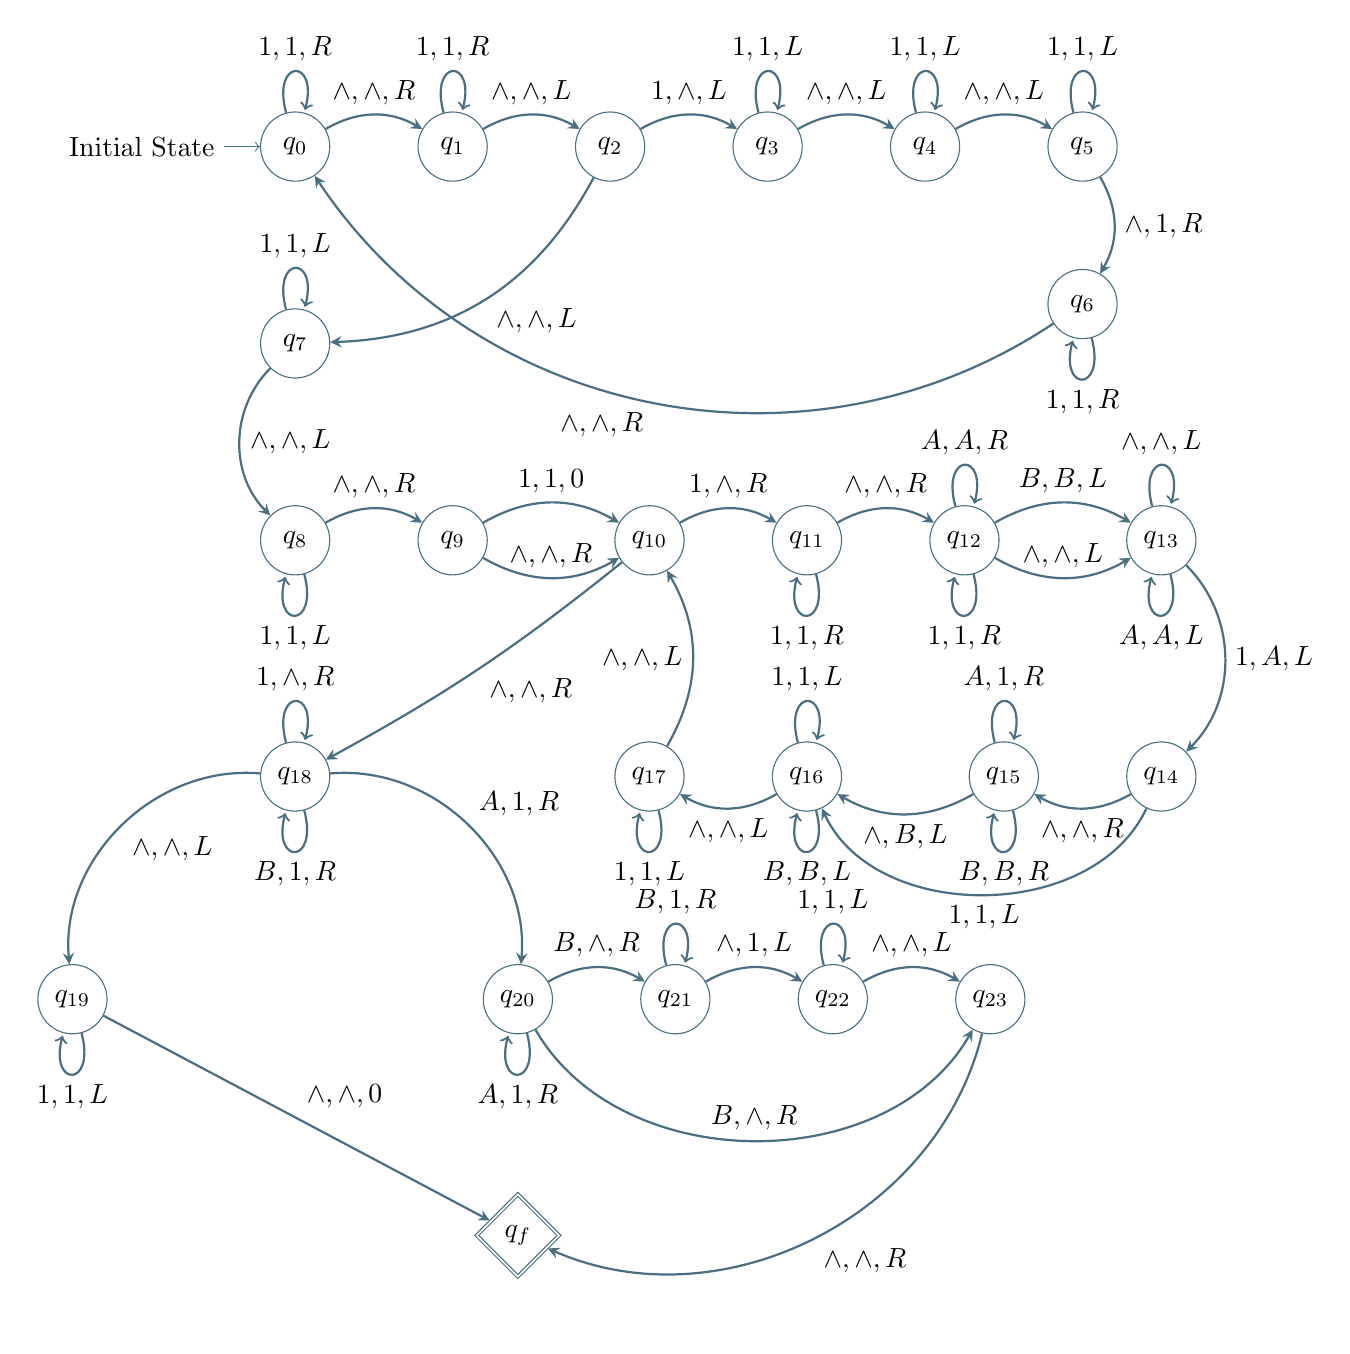
\begin{tikzpicture} [draw=cyan!45!black,
            node distance = 2cm, 
            on grid, 
            auto]
        
        % State q0
        \node (q0) [state, 
            initial,  
            initial text = {Initial State}] {$q_0$};

        % State q1    
        \node (q1) [state,
            right = of q0] {$q_1$};

        % State q2    
        \node (q2) [state,
            right = of q1] {$q_2$};        

        % State q3    
        \node (q3) [state,
            right = of q2] {$q_3$};        

        % State q4    
        \node (q4) [state,
            right = of q3] {$q_4$};

        % State q5    
        \node (q5) [state,
            right = of q4] {$q_5$};

        % State q6    
        \node (q6) [state,
            below = of q5] {$q_6$};

        % State q7    
        \node (q7) [state,
            below =2.5cm and of q0] {$q_7$};    
            
        % State q8    
        \node (q8) [state,
            below = 2.5cm and of q7] {$q_8$};    
            
        % State q9    
        \node (q9) [state,
            right = of q8] {$q_9$};  
            
        % State q10    
        \node (q10) [state,
            right = 2.5cm of q9] {$q_{10}$};  
              
            
        % State q11    
        \node (q11) [state,
            right = of q10] {$q_{11}$};  
                    
        % State q12    
        \node (q12) [state,
            right = of q11] {$q_{12}$};  
                              
        % State q13    
        \node (q13) [state,
        right = 2.5cm of q12] {$q_{13}$};  
                      
        % State q14    
        \node (q14) [state,
        below = 3cm of q13] {$q_{14}$};  
                      
        % State q15   
        \node (q15) [state,
        left = of q14] {$q_{15}$};  
                      
        % State q16    
        \node (q16) [state,
        left = 2.5cm of q15] {$q_{16}$};  
                      
        % State q17    
        \node (q17) [state,
        left = of q16] {$q_{17}$};  
                      
        % State q18    
        \node (q18) [state,
        left = 4.5cm of q17] {$q_{18}$};  
                                
        % State q19    
        \node (q19) [state,
        below left = 4cm of q18] {$q_{19}$};  
                                          
        % State q20    
        \node (q20) [state,
        below right = 4cm of q18] {$q_{20}$};  
                                                    
        % State q21    
        \node (q21) [state,
        right = of q20] {$q_{21}$};  
                                                    
        % State q22    
        \node (q22) [state,
        right = of q21] {$q_{22}$};  
                                                    
        % State q23    
        \node (q23) [state,
        right = of q22] {$q_{23}$};  

        % State q2f    
        \node (qf) [state, diamond, accepting,
            below = 3cm of q20] {$q_{f}$}; 
        % Arrows
        \path [-stealth, thick]
            % Copying machine && Formatting
            (q0) edge [bend left] node {$\land,\land,R$} (q1)
            (q1) edge [bend left] node {$\land,\land,L$} (q2)
            (q2) edge [bend left] node {$1,\land,L$} (q3)
            (q2) edge [bend left] node {$\land,\land,L$} (q7)
            (q3) edge [bend left] node {$\land,\land,L$} (q4)
            (q4) edge [bend left] node {$\land,\land,L$} (q5)
            (q5) edge [bend left] node {$\land,1,R$} (q6)
            (q6) edge [bend left=45] node {$\land,\land,R$} (q0)
            (q7) edge [bend right=45] node {$\land,\land,L$} (q8)
            (q8) edge [bend left] node {$\land,\land,R$} (q9)
            (q9) edge [bend left] node {$1,1,0$} (q10)
            (q9) edge [bend right] node {$\land,\land,R$} (q10)

            (q0) edge [loop above]  node {$1,1,R$}()
            (q1) edge [loop above]  node {$1,1,R$}()
            (q3) edge [loop above]  node {$1,1,L$}()
            (q4) edge [loop above]  node {$1,1,L$}()
            (q5) edge [loop above]  node {$1,1,L$}()
            (q6) edge [loop below]  node {$1,1,R$}()
            (q7) edge [loop above]  node {$1,1,L$}()
            (q8) edge [loop below]  node {$1,1,L$}()

            % TM
            (q10) edge [bend left] node {$1,\land,R$} (q11)
            (q10) edge [bend right=-5] node {$\land,\land,R$} (q18)
            (q11) edge [bend left] node {$\land,\land,R$} (q12)
            (q12) edge [bend left] node {$B,B,L$} (q13)
            (q12) edge [bend right] node {$\land,\land,L$} (q13)
            (q13) edge [bend left=45] node {$1,A,L$} (q14)
            (q14) edge [bend left] node {$\land,\land,R$} (q15)
            (q14) edge [bend left=65] node {$1,1,L$} (q16)
            (q15) edge [bend left] node {$\land,B,L$} (q16)
            (q16) edge [bend left] node {$\land,\land,L$} (q17)
            (q17) edge [bend right] node {$\land,\land,L$} (q10)
            (q18) edge [bend left=50] node {$A,1,R$} (q20)
            (q18) edge [bend right=50] node {$\land,\land,L$} (q19)
            (q19) edge [bend right=0] node {$\land,\land,0$} (qf)
            (q20) edge [bend left] node {$B,\land,R$} (q21)
            (q20) edge [bend right=60] node {$B,\land,R$} (q23)
            (q21) edge [bend left] node {$\land,1,L$} (q22)
            (q22) edge [bend left] node {$\land,\land,L$} (q23)
            (q23) edge [bend left=50] node {$\land,\land,R$} (qf)

            (q11) edge [loop below]  node {$1,1,R$}()
            (q12) edge [loop below]  node {$1,1,R$}()
            (q12) edge [loop above]  node {$A,A,R$}()
            (q13) edge [loop above]  node {$\land,\land,L$}()
            (q13) edge [loop below]  node {$A,A,L$}()
            (q15) edge [loop below]  node {$B,B,R$}()
            (q15) edge [loop above]  node {$A,1,R$}()
            (q16) edge [loop above]  node {$1,1,L$}()
            (q16) edge [loop below]  node {$B,B,L$}()
            (q17) edge [loop below]  node {$1,1,L$}()
            (q18) edge [loop below]  node {$B,1,R$}()
            (q18) edge [loop above]  node {$1,\land,R$}()
            (q19) edge [loop below]  node {$1,1,L$}()
            (q20) edge [loop below]  node {$A,1,R$}()
            (q21) edge [loop above]  node {$B,1,R$}()
            (q22) edge [loop above]  node {$1,1,L$}()
            ;
        \end{tikzpicture}
\end{document} % This is the end of the document
